 
\documentclass[xcolor=pdftex,dvipsnames,table]{beamer}
\usepackage{etex}
% EEHPT: You can change the theme color from Green to other colors.
\usecolortheme[named=Blue]{structure}

\usetheme{CambridgeUS}
%\usefonttheme{serif}
\setbeamercovered{dynamic}
\usepackage{wrapfig}
\usepackage[absolute,overlay]{textpos}
\usepackage{verbatim}
%\usepackage{hyperref}
\usepackage{graphicx}
\usepackage{ifthen}

    \usepackage{tikz}
    \usetikzlibrary{arrows}
	\usetikzlibrary{decorations.pathreplacing}
	\usepackage{tikz-3dplot} %requires 3dplot.sty to be in same directory, or in your LaTeX installation
	
	
\usepackage{float}
\usepackage[export]{adjustbox}
\usepackage{bm}
\usepackage{amsmath}
\usepackage{hyperref}
\usepackage{booktabs}
\newtheorem{name}{Printed output}
\newtheorem{prop}{Proposition}
\newtheorem{assum}{Assumptions}
\newtheorem{defin}{Definitions}
\newtheorem{lemm}{Lemma}
\setbeamercovered{invisible}


\begin{document}

\title{Programas de Combate \`a Pobreza \'Otimos}
\subtitle{Uma aplica\c{c}\~ao ao \textit{Bolsa Fam\'ilia}}
\author{Juan Rios}

\maketitle

\begin{frame}
 \frametitle{Introdu\c{c}\~ao}
% EEHPT: Put content here (of course, you can make it more than one slide)
\pause
\begin{itemize}
\item Impasse entre academia e pol\'itica publica:
\begin{itemize}
\item Academia: Maximizar o bem-estar social
\item Policy makers: Reduzir a pobreza
\end{itemize}
\pause
\item \textit{Bolsa Fam\'ilia} \'e o maior programa de transfer\^encia condicional de renda do mundo
\begin{itemize}
\pause
\item 30 milh\~oes de benefici\'arios em Mar\c{c}o de 2015
\pause
\item Indiv\'iduos abaixo de renda anual de US\$ 528 (EITC abaixo de US\$ 16,000)
\end{itemize}
\end{itemize}
\end{frame}

\begin{frame}[label=question]
 \frametitle{O que sabemos na academia sobre redistribui\c{c}\~ao de renda?}
% EEHPT: Put content here (of course, you can make it more than one slide)
\begin{itemize}
\item O imposto de renda que maximiza a fun\c{c}\~ao de bem-estar
\begin{itemize}
\item BF \'e um Imposto de Renda Negativo
\item Bem-estar: soma de fun\c{c}\~oes de utilidade
\item Precisamos de algumas estat\'isticas dos dados de renda (Saez, 2001)
\end{itemize}
\pause
\item Problemas 
\begin{itemize}
\item N\~ao sabemos bem como som\'ar-las.
\item No Brasil, Imposto de renda dissociado do BF
\end{itemize}
\end{itemize}
\end{frame}

\begin{frame}[label=literature]
 \frametitle{O que proponho}
% EEHPT: Put content here (of course, you can make it more than one slide) 
\begin{itemize}
\item Maximizar a renda m\'inima brasileira dado o or\c{c}amento do programa
\begin{itemize}
\item Mais pr\'oximo do objetivo real do governo
\item O que voc\^es acham?
\end{itemize}
\pause
\item Estimar as estat\'isticas necess\'arias usando os dados do BF e da RAIS
\begin{itemize}
\item Incentivos gerados pelo programa
\item Capacidade de fiscaliza\c{c}\~ao 
\end{itemize}
\end{itemize}
\end{frame}

\begin{frame}
\frametitle{Domic\'ilios com 3 membros \only<-3>{e 1 Crian\c{c}a} \only<4->{ap\'os a \'ultima reforma}}
\begin{center}
\scalebox{0.7}{
\begin{tikzpicture}[x=1.4,y=2.4]
\node[align=center, right] at (200,0) {Renda};
\draw[->, very thick] (0,0) -- (200,0) ; %edit here for the x axis
\node[align=center, above] at (0,100) {Benef\'icio};
\draw[->, very thick] (0,0) -- (0,100) ; %edit here for the y axis

\pause
\only<1-3>{\draw[blue!70!black, -] (0,70) -- (36,34) ; % flat line
\draw[blue!70!black, -] (36,34) -- (70,34); % 45 degree line
\draw[blue!70!black, -] (70,34) -- (70,10.666) ; % notch
\draw[blue!70!black, -] (70,10.666) -- (140,10.666) ; % 45 degree line
\draw[blue!70!black, -] (140,10.666) -- (140,0) ; % notch
\draw[blue!70!black, -] (140,0) -- (180, 0); % 45 degree line

\draw[blue!70!black, -] (165,100) -- (180, 100);
\node[black, align=center, right] at (180,100) {06.18.2012};
%Note that this date should be adjusted to 11.18.2012 if child is older than 6 (but younger than 15)
\node[black, align=right, left] at (0,70) {\scriptsize{70}};
\draw[black, -, dashed, thick] (70,0) -- (70,10.666) ;
\node[black, align=center, below] at (70,0) {\scriptsize{70}};
\node[black, align=center, below] at (140,0) {\scriptsize{140}};}


\pause
\only<3->{\draw[black, -] (0,77) -- (39.666,37.333) ; % flat line
\draw[black, -] (39.666,37.333) -- (77,37.333); % 45 degree line
\draw[black, -] (77,37.333) -- (77,11.666) ; % notch
\draw[black, -] (77,11.666) -- (154,11.666) ; % 45 degree line
\draw[black, -] (154,11.666) -- (154,0) ; % notch
\draw[black, -] (154,0) -- (180, 0); % 45 degree line

\draw[black, -] (165,110) -- (180, 110);
\node[black, align=center, right] at (180,110) {\only<3>{06.01.2014}\only<4->{With Children}};
\node[black, align=right, left] at (0,77) {\scriptsize{77}};
\draw[black, -, dashed, thick] (77,0) -- (77,11.666) ;
\node[black, align=center, below] at (77,0) {\scriptsize{77}};
\node[black, align=center, below] at (154,0) {\scriptsize{154}};}
\pause
\only<4->{\draw[orange, -] (0,77) -- (51.333,25.666) ; % flat line
\draw[orange, -] (51.333,25.666) -- (77,25.666); % 45 degree line
\draw[orange, -] (77,25.666) -- (77,0) ; % notch
\draw[orange, -] (77,0) -- (180, 0); % 45 degree line

\draw[orange, -] (165,100) -- (180, 100);
\node[black, align=center, right] at (180,100) {Without Children};}
\end{tikzpicture}
}
\end{center}
\end{frame}

\section{Dados}
\begin{frame}
	\frametitle{Dados}
% EEHPT: Put content here (of course, you can make it more than one slide)
\pause
\begin{itemize}
\item Cadunico para 2012-2015 (apenas 2015 hoje)
\begin{itemize}
\item Renda e renda per capita domiciliar
\item Composi\c{c}\~ao Familiar
\item Data da atualiza\c{c}\~ao
\end{itemize}
\pause
\item RAIS
\begin{itemize}
\item Renda reportada por firmas
\item M\^es de refer\^encia
\item CPF
\end{itemize}
\end{itemize}
\end{frame}

\begin{frame}
\begin{table}[htbp]
  \centering
  \caption{Quem est\'a no Mercado Formal?}
    \begin{tabular}{crr|r}
\toprule
 & Only BF & Formal Empl. & Total \\
\midrule
Individuals & 2560438 & 455495 & 3015933 \\
 & (     84.9\%) & (     15.1\%) & (100\%) \\
Hhs (1 formal empl) & 634088 & 359267 & 993355 \\
 & (     63.8\%) & (     36.2\%) & (100\%) \\
Hhs (All formal empl) & 746007 & 247348 & 993355 \\
 & (     75.1\%) & (     24.9\%) & (100\%) \\
\bottomrule
\end{tabular}

  \label{tab_selection}%
\end{table}%
\end{frame}

\begin{frame}[label=ybar0]
\frametitle{Distribui\c{c}\~ao da Renda reportada (sem filhos)}
\begin{figure}[H]
\begin{center}
\includegraphics[height=2.7in]{Dom_060114_non_0_bin3p5.pdf}
\end{center}
\end{figure}
\hyperlink{ybar0_sel}{\beamergotobutton{Link Selected Sample}}
\end{frame}

\begin{frame}[label=ybar2]
\frametitle{Distribui\c{c}\~ao da Renda reportada (2 crian\c{c}as)}
\begin{figure}[H]
\begin{center}
\includegraphics[height=2.7in]{Dom_060114_non_2_bin3p5.pdf}
\end{center}
\end{figure}
\hyperlink{ybar2_sel}{\beamergotobutton{Link to Selected Sample}}
\end{frame}

\begin{frame}
\frametitle{Distribui\c{c}\~ao da Renda formal (sem filhos)}
\begin{figure}[H]
\begin{center}
\includegraphics[height=2.7in]{Rais_060114_non_0_bin3p5.pdf}
\end{center}
\end{figure}
\end{frame}

\begin{frame}
\frametitle{Distribui\c{c}\~ao da Renda formal (2 crian\c{c}as)}
\begin{figure}[H]
\begin{center}
\includegraphics[height=2.7in]{Rais_060114_non_2_bin3p5.pdf}
\end{center}
\end{figure}
\end{frame}

\begin{frame}
\frametitle{O que preciso nos dados}
\begin{itemize}
\item Em qual tabela do BF cada domic\'ilio se encaixa?
\begin{itemize}
\item N\'umero de Membros 
\item Elig\'ivel para quais benef\'icios
\end{itemize}
\pause
\item A frequ\^encia da renda reportada e formal per capita
\begin{itemize}
\item RAIS (j\'a tenho)
\item BPC 
\item Seguro Desemprego
\item INSS
\end{itemize}
\end{itemize}
\end{frame}


\begin{frame}
\frametitle{Problemas}
\begin{itemize}
\item Renda per capita do domic\'ilio difere da tabela pessoa em 2\% das fam\'ilias (Cadunico)
\item Alguns indiv\'iduos recebem benef\'icios que n\~ao deveriam (Benef\'icios)
\end{itemize}
\end{frame}

\begin{frame}
\frametitle{Benef\'icio B\'asico para Dom. com Mais de 77 renda pc (25\%!)}
\begin{table}[htbp]
  \centering
  \caption{Benef\'icio B\'asico}
    \begin{tabular}{rrrrr}
    \toprule
    idHh  & idInd & dta\_atual\_memb & rf\_folha & ben. Basico \\
    \midrule
    137   & 16033997884 & 2014-08-06 & 3/1/15 & 77 \\
    \bottomrule
    \end{tabular}
\end{table}%
\end{frame}

\begin{frame}
\frametitle{Benef\'icios}
% Table generated by Excel2LaTeX from sheet 'Sheet1'
\begin{table}[htbp]
  \centering
  \caption{Benef\'icio de 0 a 6}
  \scalebox{0.6}{
    \begin{tabular}{rrrrrrrr}
    \toprule
    idHh  & idInd & dta\_atual\_memb & dta\_nasc\_pessoa & idade (Cad) & rf\_folha & idade (Folha) & benefit0to6 \\
    \midrule
    389059 & 16052941988 & 2015-02-02 & 1995-04-04 & 19    & 2/1   & 19    & 35 \\
    \bottomrule
    \end{tabular}}
\end{table}
\end{frame}

\begin{frame}
\frametitle{Benef\'icios de 7 a 15 (muito novo)}
\begin{table}[htbp]
  \centering
  \caption{Benef\'icio de 7 a 15}
    \scalebox{0.6}{
    \begin{tabular}{rrrrrrrr}
    \toprule
    idHh  & idInd & dta\_atual\_memb & dta\_nasc\_pessoa & idade (Cadunico) & dateFolha & idade (Folha) & benefit7to15 \\
    \midrule
    2793  & 16324772234 & 2011-02-01 & 2008-03-12 & 2     & 3/15 & 6     & 35 \\
    \bottomrule
    \end{tabular}}
\end{table}%
\end{frame}

\begin{frame}
\frametitle{Benef\'icios de 7 a 15 (muito velho)}
\begin{table}[htbp]
  \centering
  \caption{Benef\'icio de 7 a 15}
      \scalebox{0.6}{
    \begin{tabular}{rrrrrrrr}
    \toprule
    idHh  & idInd & dta\_nasc\_pessoa & dta\_atual\_memb & idade (Cad) & dateFolha & idade (Folha) & benefit7to15 \\
    \midrule
    38833 & 16038377272 & 1999-02-04 & 2015-02-04 & 16    & 2/1/15 & 16    & 35 \\
    \bottomrule
    \end{tabular}}
\end{table}%
\end{frame}

\begin{frame}
\frametitle{\'Ultimas Perguntas}
\begin{itemize}
\item Como identificam nutrizes na base?
\item Como identificam gr\'avidas na base?
\item Como identificam gr\'avidas na base?
\end{itemize}
\end{frame}

\begin{frame}
Muito obrigado!
\end{frame}

\appendix
\newcounter{finalframe}
\setcounter{finalframe}{\value{framenumber}}

\begin{frame}[label=ybar0_sel]
\frametitle{Reported Income  (0 children) - Selected Sample}
\begin{figure}[H]
\begin{center}
\includegraphics[height=2.7in]{Dom1_060114_non_0_bin3p5.pdf}
\end{center}
\end{figure}
\hyperlink{ybar0}{\beamergotobutton{Back to Households with 0 Children}}
\end{frame}

\begin{frame}[label=ybar2_sel]
\frametitle{Reported Income (2 children) - Selected Sample}
\begin{figure}[H]
\begin{center}
\includegraphics[height=2.7in]{Dom1_060114_non_2_bin3p5.pdf}
\end{center}
\end{figure}
\hyperlink{ybar2}{\beamergotobutton{Back to Complete Sample}}
\end{frame}

\begin{frame}[label=proof_empirical]
\begin{itemize}
\item $y^*_{jt}=\sum_{i=1}^I d_{ij}(w_i*h_{i,j,t}+ w_{i-1}* h_{i-1,j,t})+\lambda_1+u_{jt},$
\item $h_{ijt}=\begin{cases}1$ if $h_{ijt}^*>0\\
0$ otherwise,$\end{cases}\ where\ h^*_{ijt}=f(\underbrace{(c_i-c_0),(c_i-c_{i-1})}_{X_{jt}})+\epsilon_{ijt},$
\item $E(h_{ijt}|X_{jt})=Prob(h_{ijt}^*=1|X_{jt})=Prob\Big(\epsilon_{ijt}>-f(X_{ijt})\Big)=1-G\Big(f(X_{ijt})\Big)$
\item $\Rightarrow h_{ijt}=1-G(f(X_{ijt}))+\lambda_2+\nu_{ijt}$
\item $y^*_{jt}=\sum_{i=1}^I \beta_i d_{ij}ln(c_i-c_{i-1})_{jt}+\sum_{i=1}^I \gamma_i d_{ij}ln(c_i-c_{0})_{jt}+\lambda+v_{jt}$\\
\begin{align*}
\beta=\frac{\partial E(y^*_{jt}|d_{ij}=1)}{\partial ln(c_i-c_{i-1})_{t}}= w_i\frac{\partial E(h_{i,j,t}|d_{ij}=1)}{\partial ln(c_i-c_{i-1})_{t}} \\
\eta_i = \frac{1}{P(h_{ij}=1)}\beta
\end{align*}
\end{itemize}
\hyperlink{empirical_relation}{\beamergotobutton{Back to Empirical}}
\end{frame}

\begin{frame}[label=theory]
 \frametitle{Theoretical Framework}
 \begin{center}
$U^E=w_{\bar{i}+\tilde{i}}+B_{\bar{i}}-p_{\bar{i}}f_{\tilde{i}}-\psi(\bar{i}+\tilde{i},\tilde{i},m)$ 
 \end{center}
\pause
\begin{itemize}
\item $\bar{i}$: reported income level 
\item $\tilde{i}$: hidden income level $\Rightarrow \bar{i}+\tilde{i}$ real income level
\item $w_0=0<w_1<...<w_I$: wages in each income level 
\pause
\item $B_0,B_1,...,B_I$: Benefits for each reported level
\pause
\item $p_{\bar{i}}$: probability of being audited if reports $\bar{i}$
\item $f_{\tilde{i}}$: fine of hiding $\tilde{i}$
\pause
\item $\psi(\cdot,\cdot,m)$: Labor supply and misreporting costs of types $m$.
\end{itemize}
\pause
 \begin{assum}
\begin{enumerate}
\item No income effect. 
\item Expected utility 
\item Some types cannot work
\pause
\item Type $m$ reports either level $0$, $i(m)-1$ or $i(m)$:
\end{enumerate}
\end{assum}
\hyperlink{implications}{\beamergotobutton{Back to Implications}}
\end{frame}

\begin{frame}[label=imp]
 \frametitle{Cost Minimizing Objective}
\begin{itemize}
\item $\bar{h}_i$: Proportion of households reporting level $i$ in equilibrium
\item $\tilde{h}_i$: Proportion of households producing $i$ but reporting $i-1$.
\item $\tilde{H}_i$: Proportion of households producing $i$ but reporting $0$.
\pause
\item $c_i=w_i+B_i$: Consumption observed by the government
\pause
\item $z$: Minimum Consumption Level.
\pause
\begin{align*}
	\underset{\{B_i\}_{i=0}^I}{min} \sum_{i=0}^I \{\bar{h}_iB_i-p_{i-1}f_1\tilde{h}_i-p_0f_i\tilde{H}_i\} \nonumber\\
	st\ c_0 \geq z\ and\ B_i\geq0\ \forall i. \nonumber
\end{align*}
\end{itemize}
\end{frame}

\begin{frame}[label=elasticities]
\begin{defin}
	Reported income elasticity in the extensive margin:
	\begin{align*}
	\bar{\eta}_i \equiv \frac{c_i-c_0}{\bar{h}_i}\frac{\partial \bar{h}_i}{\partial (c_i-c_0)},
\end{align*}
Reported income elasticity in the intensive margin:
\begin{align*}
	\bar{\mathcal{E}}_i \equiv \frac{c_i-c_{i-1}}{\bar{h}_i}\frac{\partial \bar{h}_i}{\partial (c_i-c_{i-1})}.
\end{align*}
\end{defin}
\end{frame}

\begin{frame}
$h_i$: Proportion of households producing $i$.
\pause
\begin{defin}
	Real income elasticity in the extensive margin:
	\begin{align*}
	\eta_i \equiv \frac{c_i-c_0}{h_i}\frac{\partial h_i}{\partial (c_i-c_0)},
\end{align*}
Real income elasticity in the intensive margin:
\begin{align*}
	\mathcal{E}_i \equiv \frac{c_i-c_{i-1}}{h_i}\frac{\partial h_i}{\partial (c_i-c_{i-1})}.
\end{align*}
\end{defin}
\hyperlink{implications}{\beamergotobutton{Back to Implications}}
\end{frame}

\begin{frame}[label=prop_imp]
\begin{prop}
	\label{prop_imp_tra}
	Assuming that $\hat{\eta}^{*}_i\leq \frac{c^*_i-z}{z}$ for $i\geq v$, the cost minimizing schedule $\{B^*_i\}_{i=0}^I$ is: 
	\begin{align*}
	B_0^* = z \nonumber\\		
	\frac{B_i^*-B_{i-1}^*}{c^*_i-c^*_{i-1}}=-\frac{1}{\hat{\mathcal{E}}^*_i}\sum_{j=i}^{I}\left(\bar{h}^*_j+\hat{\eta}^*_i\frac{B_j^*-z}{c^*_j-z}\right)\	 for\ i =1,...,v-1  \nonumber\\
	B^*_i = 0\ for\ i = v, v+1, ...,I. \nonumber
	\end{align*}
	Where $\hat{\eta}^*_i\equiv(1-M_{\bar{n}(i)})h^*_i\eta^{*}_i+M_{\bar{n}(i)}\bar{h}^*_i\bar{\eta}^*_i$, 
	$\hat{\mathcal{E}}^*_i\equiv(1-\mu_{\bar{m}(i)})h^*_i\mathcal{E}^{*}_i+\mu_{\bar{m}(i)}\bar{h}^*_i\bar{\mathcal{E}}^*_i$ and $v$ is the smallest $i$ such that the $B^*_i$ implied by the second bracket is less or equal to zero. 
\end{prop}
\hyperlink{implications}{\beamergotobutton{Back to Implications}}
\hyperlink{proof_main}{\beamergotobutton{Link to Proof}}
\hyperlink{lemma}{\beamergotobutton{Link to Lemma}}
\hyperlink{welfare}{\beamergotobutton{Link to Welf Prob}}
\hyperlink{efficiency}{\beamergotobutton{Link to Efficiency}}
\begin{block}

\textbf{Problem:} Elasticities under the optimal schedule $\Rightarrow$ Non-recoverable.
\end{block}
\end{frame}

\begin{frame}[label=reform]
\begin{prop}
The cost minimizing local reform is a vector of perturbation in the benefit schedule $\Delta B = -(C_0,..,C_I)$ where:
	\begin{align*}				
	 C_0 =\begin{cases}\bar{h}_0-\sum_{i=1}^{v-1}\frac{B_i-B_0}{c_i-c_0}\hat{\eta}_i\ & if\ B_0>z\\
	 0\ & if\ B_0=z \end{cases}\\
	 C_i =\bar{h}_i+\frac{B_i-B_0}{c_i-c_0}\hat{\eta}_i+\frac{B_i-B_{i-1}}{c_i-c_{i-1}}\hat{\mathcal{E}}_i-\frac{B_{i+1}-B_{i}}{c_{i+1}-c_{i}}\hat{\mathcal{E}}_{i+1}\ 1\leq i\leq v\\ for\ \ i =1,...,v-1\\
	 C_{i} =min\left\{\bar{h}_{i}-\frac{B_0}{c_{i}-c_0}\hat{\eta}_{i}-\frac{B_{i-1}}{c_{i}-c_{i-1}}\hat{\mathcal{E}}_{i},0\right\}\ for\ i=v,...,I
	\end{align*}
	 $v$: lowest level with zero benefits
\end{prop}	
\pause
\begin{block}

\textbf{Here all the parameters are recoverable from the data.}
\end{block}
\hyperlink{implications}{\beamerbutton{Back to Implications}}
\end{frame}

\begin{frame}[label=proof_main]
\begin{proof}
Since there are households that cannot work $\Rightarrow B_0^*=z$ \\
\pause
Consider the perturbation at the optimum $dB_i=dB_{i+1}=...=dB_I=dB$. \\
\begin{enumerate}
\pause
\item $ME =  dB\sum_{j=i}^Ih_j$.\\
\pause
\item $BEIM = dh^{int}_i(B_i-B_{i-1})= (dk^{int}_i-de_i)(B_i-B_{i-1})$\\
\pause
\item $BEEM = \sum_{j=i}^Idh^{ext}_j(B_j-B_0) =\sum_{j=i}^I(dk^{ext}_j-dE_j)(B_j-B_0) $\\
\pause
\item $FE =-p_{i-1}f_1de_i-p_{0}\sum_{j=i}^If_jdE_j$\\
\end{enumerate}
\pause
At the optimum: $ME + BEIM + BEEM +FE= 0$.
\pause
\begin{align*}
BEIM+FEIM=dk^I_i(B_i-B_{i-1})+de_i[(B_{i-1}-B_{i})-p_{i-1}f_1]=\\
dk^I_i(B_i-B_{i-1})+de_i\mu_{\bar{m}(i)}(B_{i-1}-B_{i})=\\
\left[(1-\mu_{\bar{m}(i)})dk^I_i+\mu_{\bar{m}(i)} dh_i^I\right](B_i-B_{i-1})
\end{align*} 
\pause
$\bar{\eta}^{*}_i\leq \frac{c^*_i-z}{z}$  for $i>v$ ensures  $B^*_{i-1}\geq B^*_i$ and hence $B^*_i=0$.
\end{proof}
\hyperlink{prop_imp}{\beamergotobutton{Back to Proposition}}
\end{frame}

\begin{frame}[label=lemma]
\begin{align*}
U^E=w_{i+\tilde{i}}+B_{i}\underbrace{-p_if_{\tilde{i}}}_{transfer\ cost}-\psi(i+\tilde{i},\underbrace{\tilde{i}}_{util.\ cost}, m)
\end{align*} 
\begin{itemize}
\item   $\bar{m}(i)$ indifferent between reporting $i$ and $i-1$, given real income is $i$
\item  $\bar{n}(i)$ indifferent between reporting $i$ and $0$, given real income is $i$
\item $\mu_{\bar{m}(i)}\equiv \frac{\psi(i,1,\bar{m})-\psi(i,0,\bar{m})}{p_if_1+\psi(i,1,\bar{m})-\psi(i,0,\bar{m})}$: Share of utility cost in the int. margin
\item $M_{\bar{n}(i)}\equiv \frac{\psi(i,i,\bar{n})-\psi(i,0,\bar{n})}{p_0f_i+\psi(i,i,\bar{n})-\psi(i,0,\bar{n})}$: Share of utility cost in the ext. margin
\end{itemize}
\begin{lemm}
\label{lemma_mu}
The wedge between the marginal benefit and marginal fine cost of misreporting (the marginal utility cost) can be written as:\\
	$(B_{i-1}-B_i)-p_{i-1}f_1=(B_{i-1}-B_i)\mu_{\bar{m}(i)}$\\
	$(B_{0}-B_i)-p_0f_{i}=(B_{0}-B_i)M_{\bar{n}(i)}$\\ 
\end{lemm}
\end{frame}

\begin{frame}[label=proof_lemma]
\begin{proof}
\begin{align*}
w_i+B_{i-1}-p_{i-1}f_1-\psi(i,1,\bar{n})=w_i+B_i-\psi(i,0,\bar{n})\\
\Rightarrow (B_{i-1}-B_i)-p_{i-1}f_1= \psi(i,1,\bar{n})-\psi(i,0,\bar{n})
\end{align*}
Multiplying the RHS by $\frac{B_{i-1}-B_i}{p_{i-1}f_1+\psi(i,1,\bar{n})-\psi(i,0,\bar{n})}$, we get the 1st relation.
\begin{align*}
w_i+B_{0}-p_{0}f_i-\psi(i,i,\bar{n})=w_i+B_i-\psi(i,0,\bar{n})\\
\Rightarrow (B_{0}-B_i)-p_{0}f_i= \psi(i,i,\bar{n})-\psi(i,0,\bar{n})
\end{align*}
Multiplying the RHS by $\frac{B_{0}-B_i}{p_{0}f_i+\psi(i,i,\bar{n})-\psi(i,0,\bar{n})}$, we get the 1st relation.
\end{proof}
\hyperlink{prop_imp}{\beamergotobutton{Back to Proposition}}
\end{frame}

\begin{frame}[label=welfare]
 \frametitle{Welfarist Objective}
\begin{itemize}
\item $\delta^m$: Welfare weight on households of type $m$
\pause
\item $\tilde{i}$: hidden income so that $i+\tilde{i}$ is the real income level
\pause
\item $v(m)$: Measure of households with type $m$. 
\pause
\item $R$: Anti-poverty program's budget
\pause
\item The government solves:
\begin{align*}
\underset{\{B_0,B_1,...,B_I\}}{max} \int_M \delta^m u^m(w_{i+\tilde{i}}+B_i,i+\tilde{i},\tilde{i})dv(m)\\
subject\ to\ \sum_i h_iB_i \leq R\ and\ B_i\geq 0\ \forall i\nonumber
\end{align*}
\end{itemize}
\end{frame}

\begin{frame}[label=prop_wel]
\begin{prop}
	\label{prop_welfare}
	Assuming that $\eta^{*}_i\leq (1-g^*_i)\frac{c^*_i-B_0^*}{B_0^*}$ for $i>v$ and that there are no income effects, the welfare maximizing schedule $\{B^*_i\}_{i=0}^I$ is:
	\begin{align*}	
	\frac{B_i^*-B_{i-1}^*}{c^*_i-c^*_{i-1}}=-\frac{1}{h^*_i\mathcal{E^*}_i}\sum_{j=i}^{I}h^*_j\left(1-g^*_j+\frac{\eta^*_j(B_j^*-B_0^*)}{c^*_j-c_0^*}\right)\ for\ i =1,...,v-1\\
	B^*_i = 0\ for\ all\ i = v, v+1, ...,I \nonumber\\
	such\ that\ \sum_{i=0}^I h^*_i B^*_i = R. \nonumber
	\end{align*}
	Where $g_i=\frac{1}{h_i}\int_{m:i(m)=i} \delta^m \frac{\partial u^m(w_{i+\tilde{i}}+B_i,i+\tilde{i},\tilde{i})}{\partial c_i} dv(m)$ and $v$ is the smallest $i$ such that the $B^*_i$ implied by the second bracket is less or equal to zero. 
\end{prop}
\end{frame}

\begin{frame}[label=proof_welfare]
\begin{proof}
FOC: $\int_{M^*_i}\delta^m \frac{\partial u^m(w_{i+\tilde{i}}+B^*_i,i+\tilde{i},\tilde{i})}{\partial c_i}dv(m)-p\left[h_i^*+\sum_{j=0}^IB_j^*\frac{\partial hj^*}{\partial c_i}\right]=0$ \\
Let $g_i=\frac{1}{p h_i}\int_{M_i} \delta^m \frac{\partial u^m(w_{i+\tilde{i}}+B_i,i+\tilde{i},\tilde{i})}{\partial c_i} dv(m)$\\
FOC becomes: $(1-g_i)h_i^*=-\Big[(B_i-B_0)\frac{\partial h_i}{\partial (c_i-c_0)}+$\\
$(B_i-B_{i-1})\frac{\partial h_i}{\partial(c_i-c_{i-1})}-(B_{i+1}-B_{i})\frac{\partial h_{i+1}}{\partial(c_{i+1}-c_{i})}\Big]$\\
Summing over $i$, we get the first equation of the proposition.\\
$\eta^{*}_i\leq (1-g^*_i)\frac{c^*_i-B_0^*}{B_0^*}$ for all $i>v$ guarantees that the incremental benefits are negative for these income levels.
\end{proof}
\end{frame}

\begin{frame}[label=sufficient_wel]
\frametitle{Why the Reported Income is the Sufficient Statistic  for the Welfarist Problem?}
\begin{itemize}
\item The Optimal Anti-Poverty Program Problem has three parts: 

\begin{enumerate}
\item Distorting incentives with marginal taxes: \\
Workers already maximizing 
$\Rightarrow$ Second Order Effects

\item Government Revenue: \\
It depends on Reported Income
\item Targeting low ability people: \\
The reported income is the targeting instrument
\end{enumerate}
\end{itemize}
\hyperlink{prop_imp}{\beamergotobutton{Back to Proposition}}
\end{frame}

\begin{frame}[label=efficiency]
	\frametitle{Efficiency of Cost Minimizing Allocation}
% EEHPT: Put content here (of course, you can make it more than one slide)
\begin{itemize}
\item The objective function is concerned with income and not welfare  
\pause
\item If the poorest cannot work, caring about his income is equivalent to caring about his utility
\pause
\item Equivalent to a Rawlsian Social Planner with a budget equal to the minimum cost
\end{itemize}
\end{frame}

\begin{frame}[label=imp_literature]
\begin{table}[htbp]
  \centering
  \caption{Income Maintenance Objectives}
    \begin{tabular}{l|cc}
    \toprule
    Gov. cares for\textbackslash{} Productive & Everyone & Not Everyone \\
    \midrule
    Only Poorest & Not Efficient & Efficient \\
    Below Poverty Line & Not Efficient & Not Efficient \\
    \bottomrule
    \end{tabular}
\end{table}
\hyperlink{prop_imp}{\beamergotobutton{Back to Proposition}}
\end{frame}

\begin{frame}[label=eitc]
\begin{prop}
\label{prop_extensive}
	Assuming that households respond only in the extensive margin, the optimal transfer program would be: 
	\begin{align*}
	B_0^* = z, \nonumber\\		
		\frac{B^*_i-B^*_{0}}{c^*_i-c^*_{0}}=\frac{1}{\eta^*_i}(g_i^*-1),\\
	B^*_i = 0\ for\ all\ i = v, v+1, ...,I. \nonumber 
	\end{align*}
	Where $v$ is the smallest $i$ such that the $B^*_i$ implied by the second bracket is less or equal to zero. 
\end{prop}
Implications
\begin{enumerate}
\item If $g_i^*>1$ EITC is optimal ($B^*_1>B^*_0$)
\item EITC is never cost minimizing ($g_i^*=0$ for all $i>0$)
\end{enumerate}
\end{frame}

\begin{frame}
\frametitle{Welfare Maximizing}
\begin{figure}[H]
\begin{center}
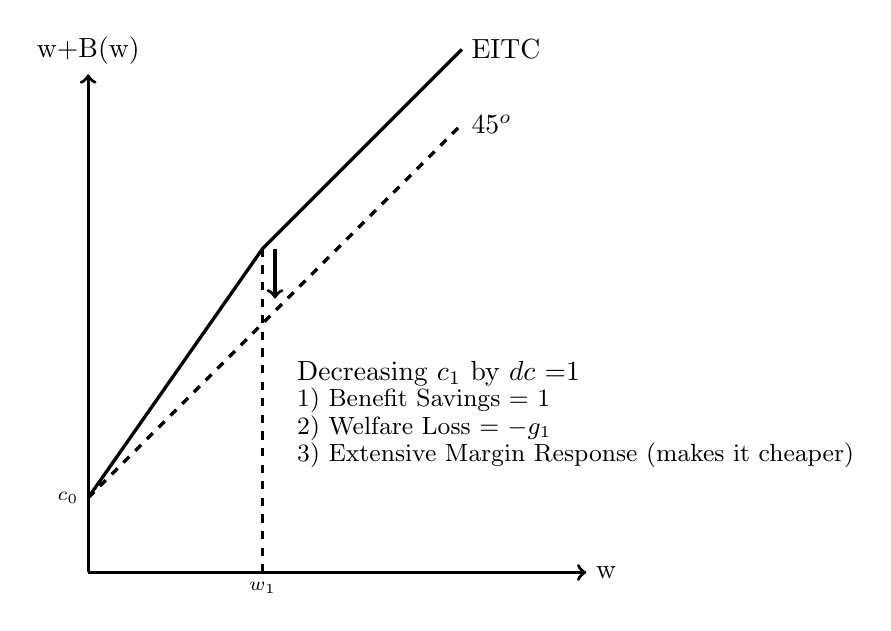
\begin{tikzpicture}[x=.9,y=.9]
\node[align=center, right] at (200,0) {w};
\draw[->, very thick] (0,0) -- (200,0) ; %edit here for the x axis
\node[align=center, above] at (0,200) {w+B(w)};
\draw[->, very thick] (0,0) -- (0,200) ; %edit here for the y axis

\draw[black, -, very thick] (0,30) -- (70,130) ; % 45 EITC
\draw[black, -, very thick] (70,130) -- (150, 210); % EITC
\node[black, align=center, right] at (150,210) {EITC};

\draw[black, -, dashed, thick] (70,0) -- (70,130) ;

\draw[->, very thick] (75,130) -- (75,110) ; %change

\draw[black, dashed, very thick] (0,30) -- (150,180) ; % 45 degree line
\node[black, align=center, right] at (150,180) {45$^o$};

\node[black, align=center, below] at (70,0) {\scriptsize{$w_1$}};

\node[black, align=right, left] at (0,30) {\scriptsize{$c_0$}};

\node[black, align=right, right] at (80,80) {Decreasing $c_1$ by $dc$ =1};
\node[black, align=right, right] at (80,69) {\small{1) Benefit Savings = 1}};
\node[black, align=right, right] at (80,58) {\small{2) Welfare Loss = $-g_1$}};
\node[black, align=right, right] at (80,47) {\small{3) Extensive Margin Response (makes it cheaper)}};
\end{tikzpicture}
\label{extensive_intuition}
\end{center}
\end{figure}
\end{frame}

\begin{frame}
\frametitle{Cost Minimizing}
\begin{figure}[H]
\begin{center}
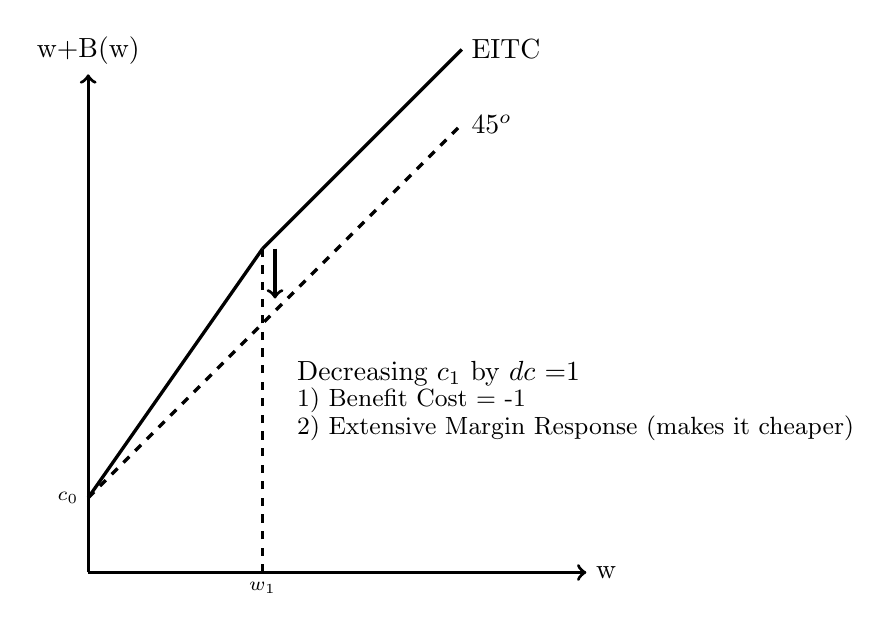
\begin{tikzpicture}[x=.9,y=.9]
\node[align=center, right] at (200,0) {w};
\draw[->, very thick] (0,0) -- (200,0) ; %edit here for the x axis
\node[align=center, above] at (0,200) {w+B(w)};
\draw[->, very thick] (0,0) -- (0,200) ; %edit here for the y axis

\draw[black, -, very thick] (0,30) -- (70,130) ; % 45 EITC
\draw[black, -, very thick] (70,130) -- (150, 210); % EITC
\node[black, align=center, right] at (150,210) {EITC};

\draw[black, -, dashed, thick] (70,0) -- (70,130) ;

\draw[->, very thick] (75,130) -- (75,110) ; %change

\draw[black, dashed, very thick] (0,30) -- (150,180) ; % 45 degree line
\node[black, align=center, right] at (150,180) {45$^o$};

\node[black, align=center, below] at (70,0) {\scriptsize{$w_1$}};

\node[black, align=right, left] at (0,30) {\scriptsize{$c_0$}};

\node[black, align=right, right] at (80,80) {Decreasing $c_1$ by $dc$ =1};
\node[black, align=right, right] at (80,69) {\small{1) Benefit Cost = -1}};
\node[black, align=right, right] at (80,58) {\small{2) Extensive Margin Response (makes it cheaper)}};
\end{tikzpicture}
\label{extensive_intuition}
\end{center}
\end{figure}
\hyperlink{prop_imp}{\beamergotobutton{Back to Proposition}}
\end{frame}

\begin{frame}[label=proof_relation]
\begin{proof}
Consider $dB_i=...=dB_I=dB$. 
The change in the cost of the program due to intensive margin responses in the discrete model is:
\begin{align*}
(B_{i-1}-B_i)dh_i-f_1de_i=[(1-\mu_{\bar{m}})dk_i+\mu_{\bar{m}} dh_i](B_{i-1}-B_i)=\\
[(1-\mu_{\bar{m}})\mathcal{E}_i^Rk_i+\mu_{\bar{m}}\mathcal{E}_ih_i]\frac{B_i-B_{i-1}}{w_i-w_{i-1}}\frac{dB}{c_i-c_{i-1}}(w_i-w_{i-1})
\end{align*}
In the continuous model, let $b_i=\frac{B_i-B_{i-1}}{w_i-w_{i-1}}$ and $f_i=\frac{p_{i-1}f_1}{w_i-w_{i-1}}$ be the marginal benefit and expected fines faced by individual with $\bar{y}=w_i$. The same perturbation $db_i=dB/(w_i-w_{i-1})$ will reduce the reported income of individuals reporting $w_i$ by $d\bar{y}=dy-d\tilde{y}$. So the tolal effect on cost is:
\begin{align*}
\{(1-\mu_{\bar{m}})[wi+\tilde{y}(w_i,m)]e_i+\mu_{\bar{m}}\bar{e}_i\}\frac{db_i}{1+b_i}h_ib_i
\end{align*}
Equating the terms multiplying $(1-\mu_{\bar{m}})$ and $\mu_{\bar{m}}$, we get the relations. 
\end{proof}
\hyperlink{discretized}{\beamergotobutton{Back to Discretized Schedule}}
\end{frame}

\setcounter{framenumber}{\value{finalframe}}

\end{document}
